

%%%%%%%%%%%%%%%%%%%%%%%%%%%%%%%%%%%%%%%%%%%%%%%%%%%%%%%%%%%%%%%%%%%%%%%%%%%%%%%%%%%%%%%%%%%%%%%%%%%%%%%%%%%%%%%%%%%%%%%%%%%%%%%%
%
%
%                   Bilateral Control Chapter  !!
%
%     


\chapter{Bilateral Control}

%%%%%%%%%%%%%%%%%%%%%%%%%%%%%%%%%%%%%%%%%%%%%%%%%%%%%%%%%%%%%%%%%%%%%%%%%%%%%%%%%%%%%%%%%%%%%%
%
%
%                Combined Systems and Networks
%
%


%\begin{slide}

\section*{Kinesthetic Interaction with Teleoperation Systems}

%%%%** Section 1
\section{Introduction}
   It was recognized in the earliest efforts to implement teleoperation systems that feedback of contact forces or constraints was very valuable for task performance.  Such a system becomes quite different from a traditional control system.   In traditional control systems, the input command (desired output) is a static value which is not influenced by any physical variable present at the output.  In a telemanipulation system with force feedback, the output state affects the input and vice-versa.   We refer to systems with this property as bi-lateral systems.   Although bi-lateral systems can be modeled with traditional block diagram or signal-flow-graph techinques, more insight is obtained with methods drawn from the theory of electrical and other networks which share this bi-lateral property.
%
In this chapter, we develop this understanding by introducing some concepts in the simplified context of a single degree of freedom bi-lateral system consisting of combined electrical, computational, communication, and mechanical components.
%
%In another chapter we expand teleoperation to multiple degrees of freedom.
%
	%<*>
%\end{slide}
%\begin{slide}
%%%%** Section 2
\section{Modeling Combined Systems}

Definitions:
\begin{itemize}

  \item {\bf Lumped Parameter Elements.}   Physical entities who's energy (storage elements) or power (dissipative elements) is defined by a scalar.

Examples:  mass:  $E = \frac{1}{2}mv^2$   resistor: $P = i^2R$

Counter Example:   Vibrating string, drum head.

  \item {\bf Network.}  A system described by lumped parameter elements connected in series and parallel.  Each element consists of one constitutive relation.

Example:   An electric circuit consisting of R, L, C in arbitrary connections.

Counter Examples:  cloud, flame, ocean wave.

   \item {\bf Port.}     A location where energy can move into or out of a network.  An effort $\ef_i$ and flow, $\fl_i$ are defined for each port.

Examples:  Electric wall socket.   Contact point between human and haptic interface.  Hydraulic coupling.

Counter Examples:  Ethernet jack.   table supporting a mass.

\end{itemize}


%\end{slide}
%\begin{slide}
%%%%** Section 2.1
\subsection{Effort and Flow}
Key insights can be obtained by focusing on energy movement within and between systems.

If energy is $E$, the time derivative of energy is power,
\bq
P = \frac{dE}{dt}
\eq
Since total energy must be conserved, power must be caused by energy moving between systems or system elements.
For  mechanical and electrical systems,
\bq
P = f \times \dot{x} \qquad      P = i \times v
\eq
We generalize the two variables which form power as  Effort ($\ef$ ) and Flow ($\fl$) respectively.
Thus
\bq
P = \ef \times \fl
\eq


% Effort: $\ef(s)$

% Flow:  $\fl(s)$

%\end{slide}
%\begin{slide}
%%%%** Section 2.2
\subsection{Impedance and Admittance}
	%<*hn>
Effort and flow variables are linked together by the behavior of systems at their ports.  Two ways to represent this relationship are impedance,
	%<*>

\bq
Z = \frac{\ef(s)}{\fl(s)}
\eq
and the admittance
\bq
A = \frac{\ef(s)}{\fl(s)} = 1/Z
\eq

%\end{slide}
%\begin{slide}




%%%%** Section 2.3
\subsection{Effort and Flow Summary}
To summarize,	%<hn>

\begin{center}
\begin{tabular}{l|l|l|l}
\hline
{\bf ``Effort"}, $\ef$  &  $\frac{dE}{dt}$         & Force              & Voltage     \\
\hline
{\bf ``Flow" },  $\fl$  &  $\frac{d}{dt}$ State    & Velocity           & Current     \\
                     &                           & ($\frac{dx}{dt}$)    & ($\frac{dq}{dt}$) \\
\hline
\end{tabular}
\end{center}

where $C$ is capacitance, $E$ is energy (or Work) and $q$ is charge. ``State" refers to a state variable such as position, $x$, and charge, $q$.

%\end{slide}
%\begin{slide}



%%%%%%%%%%%%%%%%%%%%%%%%%%%%%%%%%%%%%%%%%%%%%%%%%%%%%%%%%%%%%%%%%%%%%%%%%%%%%%%%%%%%%%%%%%%%%%%%%
%%%%** Section 3
\section{Constitutive Relations}
	%<*>
A constitutive relation is a function which relates effort to either flow, the integral of flow, or its derivative.

 In the study of linear systems, we assume the constitutive relations are linear functions, but this is not required in general.	%<hn>

 The six basic linear constitutive relations are given in Figs \ref{ConstitRelationsDissipative} and \ref{ConstitRelationsStorage}.	%<hn>

%\end{slide}
%\begin{slide}

%      (1)
%%%%** Figure 1
\begin{figure}[h]	%<hn>
\centering 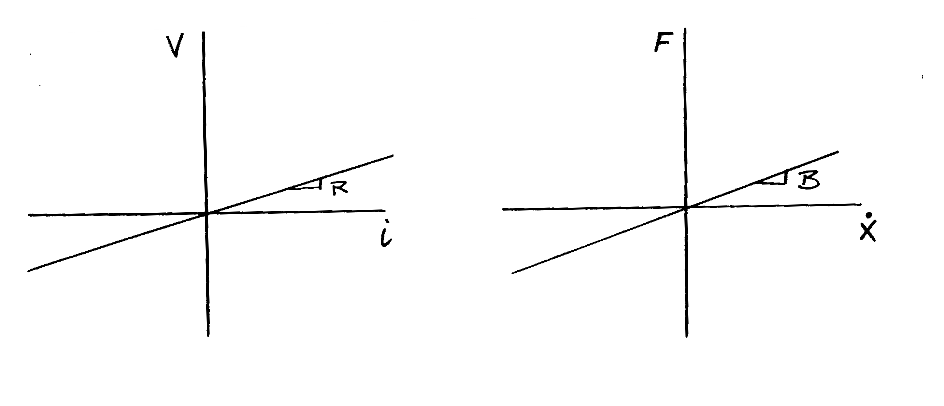
\includegraphics[width=3.5in]{figs14/00315.eps}
\caption{Constitutive relations for the linear dissipative elements resistance, $R$, and damping, $B$.}\label{ConstitRelationsDissipative}	%<hn>
\end{figure}	%<hn>


%       (2)
%%%%** Figure 2
\begin{figure}[h]	%<hn>
\centering 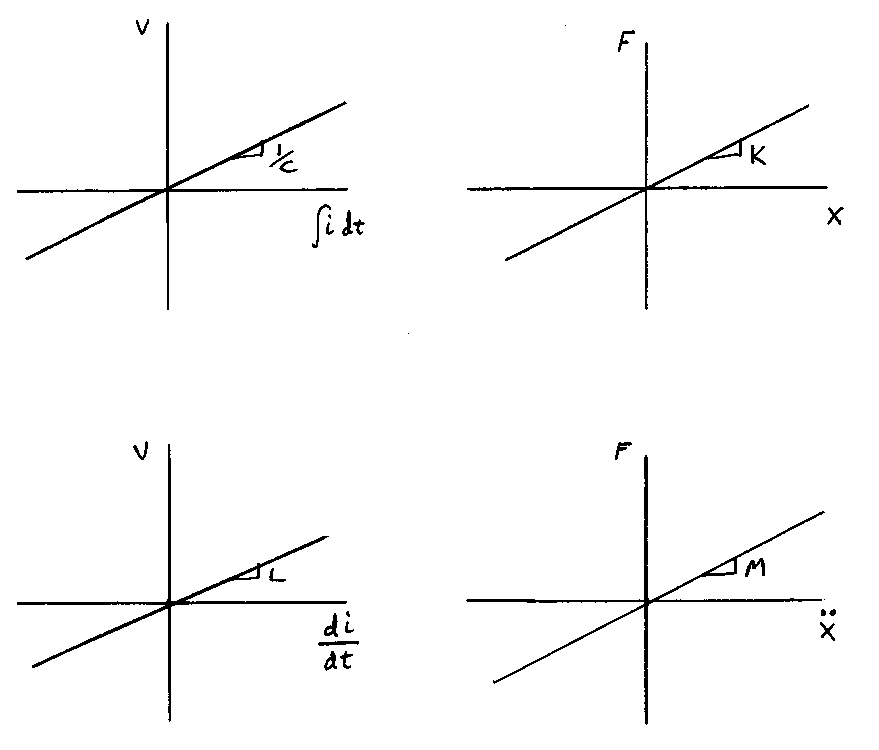
\includegraphics[width=3.5in]{figs14/00316.eps}
\caption{Constitutive relations for the linear energy storage elements, capacitance, $C$, stiffness, $K$, inductance, $L$, and mass, $M$.}\label{ConstitRelationsStorage}	%<hn>
\end{figure}	%<hn>


%\end{slide}
%\begin{slide}
%%%%** Section 3.1
\subsection{Analogies}
 The similarity of the electrical and mechanical constitutive relations, as well as the definition of effort and flow, generate the following analogies between electrical and mechanical systems.   Additional columns can be added for hydraulic systems, thermal systems, etc.	%<hn>

\begin{tabular}{ll}
Voltage & Force\\
Current & Velocity\\
Charge & Position \\
Inductance & Mass\\
Capacitance & Stiffness\\
Resistance  & Damping \\
\end{tabular}


 In some books on dynamics and control, another analogy is given in which the table above starts off	%<*hn>

\begin{tabular}{ll}
Voltage & Velocity\\
Current & Force\\
\end{tabular}

A valid system of analysis can also be constructed based on these analogies, but the following disadvantages obtain
\begin{itemize}
  \item The notions of effort and flow cannot be abstracted to aid expansion of the analysis to other domains such as thermodynamics.
  \item Physical intuition which arises from the definition of voltage as ``Electromotive Force" is lost.
\end{itemize}

An advantage of this analysis is that it can be easier to map directly between a mechanical diagram and electrical circuit.
	%<*>



%\end{slide}
%\begin{slide}

%%%%%%%%%%%%%%%%%%%%%%%%%%%%%%%%%%%%%%%%%%%%%%%%%%%%%%%%%%%%%%%%%%%%%%%%%%%%%%%%%%%%%%%%%%%%%%%%%
%%%%** Section 4
\section{Energy Ports}

One definition of a system is simply  region of space which is isolated to some degree from the environment and which contains energy storage and dissipative elements.   At some points along the boundary between the system and environment we can identify locations at which energy may move into and out of the system.  We call these locations ports.  Such a general notion of system with a port having effort and flow variables and signs is shown in Figure \ref{GeneralPort}  	%<hn>

%%%%** Figure 3
\begin{figure}[h]	%<hn>
\centering 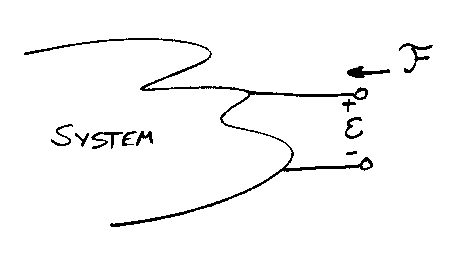
\includegraphics{figs14/00301.eps}
\caption{A port is a location where energy can be exchanged between a system and its environment described by the variables effort, $\ef$, and flow, $\fl$.}\label{GeneralPort}	%<hn>
\end{figure}	%<hn>


%\end{slide}
%\begin{slide}
%%%%%%%%%%%%%%%%%%%%%%%%%%%%%%%%%%%%%%%%%%%%%%%%%%%%%%%%%%%%%%%%%%%%%%%%%%%%%%%%%%%%%%%%%%%%%%%%%
%%%%** Section 5
\section{One-port networks}

A system which has a single port is called a one-port system or simply a one-port (Figure \ref{OnePort}).	%<hn>

%%%%** Figure 4
\begin{figure}[h]	%<hn>
\centering 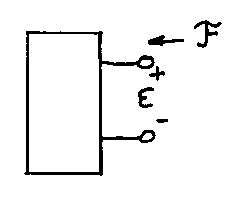
\includegraphics{figs14/00302.eps}
\caption{A one port network has a single location at which effort and flow define positive or negative power going into the network. We define the signs of effort and flow so that power is positive flowing into the port. }\label{OnePort}	%<hn>
\end{figure}	%<hn>

	%<*>
For example, a mechanical impedance is a one-port network where

\bq
\ef = F  \qquad \mathrm{and} \qquad \fl = \frac{dx}{dt} = \dot{x}
\eq

%\end{slide}
%\begin{slide}

%%%%** Section 5.1
\subsection{One Port Examples}

Example of mechanical one-port (Figure \ref{MechanicalOnePort}).	%<hn>


%          (5)
%%%%** Figure 5
\begin{figure}[p]	%<hn>
\centering 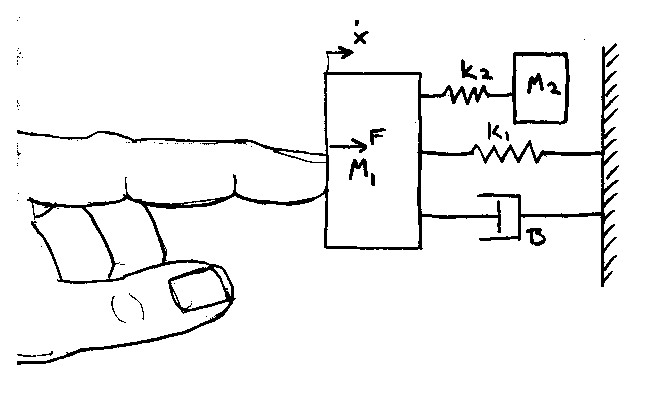
\includegraphics{figs14/00303.eps}
\caption{Example of a mechanical one-port network being touched by a fingertip.}\label{MechanicalOnePort}	%<hn>
\end{figure}	%<hn>


%\end{slide}
%\begin{slide}

\noindent Example of electrical  one-port (Figure \ref{ElectricalOnePort}).	%<hn>


%         (6)
%%%%** Figure 6
\begin{figure}[p]	%<hn>
\centering 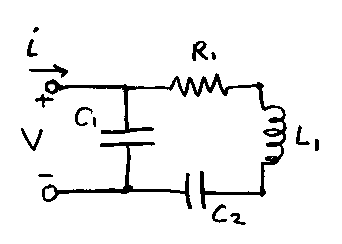
\includegraphics{figs14/00304.eps}
\caption{Example of an electrical one-port network.}\label{ElectricalOnePort}	%<hn>
\end{figure}	%<hn>


%\end{slide}
%\begin{slide}
%%%%** Section 5.2
\subsection{Vectors, Scalars, and Sign Conventions}\label{Signs}

 In mechanical systems, the effort and flow variables are often vector quantities.  In this chapter however, we simplify the system to consider scalar variables such as force and velocity in a single direction.  However just as vectors must be expressed with respect to a coordinate system, scalar effort and flow variables must be expressed with respect to a one-dimensional coordinate system which is also thought of as a sign convention.   Graphically we represent these one-dimensional coordinate systems or sign conventions with an arrow, just as with a single component of a 3 dimensional coordinate system.  In electrical network systems, the analogy to coordinate systems for current (flow) is an arrow which indicates the direction of positive current.    Voltage in networks is defined by subtracting the potential at two discrete points or terminals (and their location in space does not matter).  However we must indicate which terminal will be considered positive. 	%<hn>

It will be very important to keep track of power flowing into and out of networks so we must be careful with signs.   Signs for efforts and flows can be thought of as a simple version of a coordinate system.   Although there are multiple correct ways to do this, we will stick with the following convention:	%<hn>

%{\bf Sign Conventions}
\begin{quotation}
\noindent
1) Choose the sign of flow so that it is positive going {\it into} the port. \\
2) The effort of interest at the port is that being exerted {\it on} the port, not the effort exerted {\it by} the port on the environment.
3) Choose the sign of effort so that
\bq
\ef \times \fl > 0
\eq
when energy flows {\it into} the port.  This means that effort has the same sign as flow.
\end{quotation}

The electrical and mechanical network examples (Figures \ref{MechanicalOnePort} and \ref{ElectricalOnePort}) have sign conventions applied according to the rules above. 	%<hn>

%\end{slide}
%\begin{slide}


%\end{slide}
%\begin{slide}

%%%%** Section 5.3
\subsection{Sources}

%%%%** Figure 7
\begin{figure}[p]	%<hn>
\centering 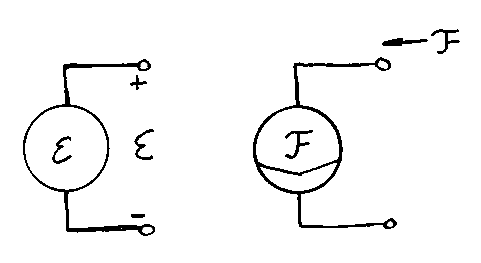
\includegraphics{figs14/00300.eps}
\caption{Effort and flow sources are one-ports which hold one variable constant.}\label{EffortFlowSources}	%<hn>
\end{figure}	%<hn>

Two additional one-port elements are effort and flow {\it sources}.    An effort source is an element for which

\bq
\ef = c
\eq
where c is a constant.   And a flow source gives
\bq
\fl = c
\eq

We can also have {\it dependent sources} which are defined above but  where $c = \alpha x$ where $x$ is another network variable.


%\end{slide}
%\begin{slide}

%%%%** Section 5.4
\subsection{Connected 1-Ports}
When two systems are connected to each other, their ports are in contact and share the effort and flow variables.  For example, consider a human operator touching a haptic interface (Figure \ref{ConnectedOnePorts}).	%<hn>

%%%%** Figure 8
\begin{figure}[p]	%<hn>
\centering 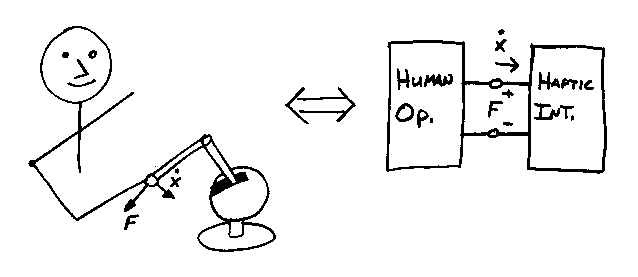
\includegraphics{figs14/00305.eps}	%<hn>
%\centering 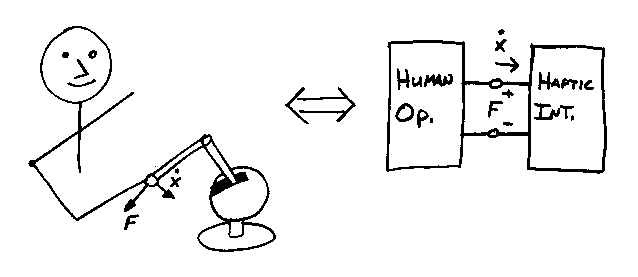
\includegraphics[width=3.5in]{figs14/00305.eps}
\caption{Human operator holding a haptic interface can be represented as two connected one-ports. In this case, the effort and flow variables are the force and velocity respectively.}\label{ConnectedOnePorts}	%<hn>
\end{figure}	%<hn>



%\end{slide}
%\begin{slide}


%%%%%%%%%%%%%%%%%%%%%%%%%%%%%%%%%%%%%%%%%%%%%%%%%%%%%%%%%%%%%%%%%%%%%%%%%%%%%%%%%%%%%%%%%%%%%%%%%
%%%%** Section 6
\section{Two-port networks}
	%<*hn>
Now we consider systems which have two ports.  We can see the need for this if we break up the haptic interface of Figure \ref{ConnectedOnePorts} to indicate the haptic device hardware, the haptic device controller, and the virtual reality model as separate components (Figure \ref{HumanHapticInterface2Ports}).  Two-ports have separate effort and flow variables, defined for each port, and a separate coordinate system (sign convention) for each port (Figure \ref{GenericTwoPort})

	%<*>
%%%%** Figure 9
\begin{figure}[p]	%<hn>
\centering 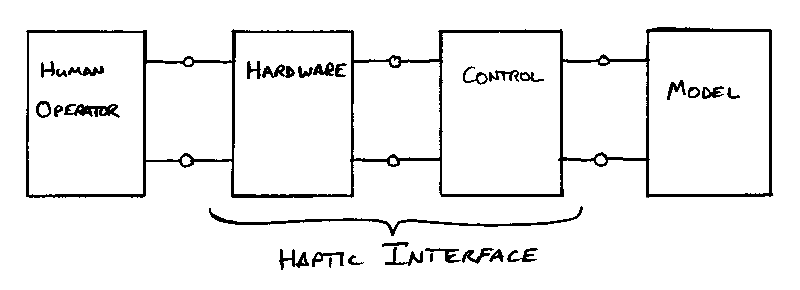
\includegraphics[width=3.5in]{figs14/00306.eps}
\caption{Expanded network diagram of human interacting with haptic interface showing haptic device hardware and haptic device controller as separate two-ports.}\label{HumanHapticInterface2Ports}	%<hn>
\end{figure}	%<hn>




%%%%** Figure 10
\begin{figure}[p]	%<hn>
\centering 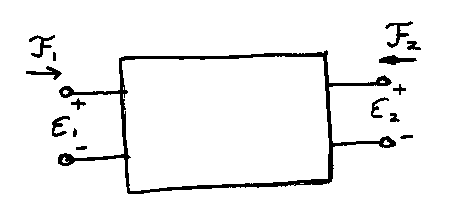
\includegraphics[width=3.5in]{figs14/00307.eps}
\caption{A two port network with effort and flow defined separately at each port.}\label{GenericTwoPort}	%<hn>
\end{figure}	%<hn>


%\end{slide}
%\begin{slide}
%%%%** Section 6.1
\subsection{Electrical Network Example: }


%%%%** Figure 11
\begin{figure}[p]	%<hn>
\centering 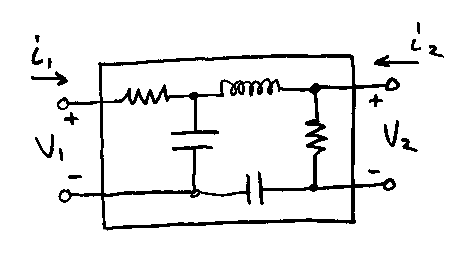
\includegraphics[width=3.5in]{figs14/00308.eps}
\caption{Example of two-port electrical network.}\label{ElectricTwoPort}	%<hn>
\end{figure}	%<hn>

	%<*hn>
In the electrical 2-port of Figure \ref{ElectricTwoPort}, $i_1$ and $i_2$ are the currents flowing {\it into} the ports at the {\it positive} terminals. When voltage and current are defined this way positive power means power flowing {\it into} the network port.

	%<*>



%\end{slide}
%\begin{slide}

%%%%** Section 6.2
\subsection{Other Notations}

%\end{slide}
%\begin{slide}
%%%%** Section 6.2.1
\subsubsection{Bond Graphs (Paynter, 1961) }


%%%%** Figure 12
\begin{figure}[h]	%<hn>
\centering 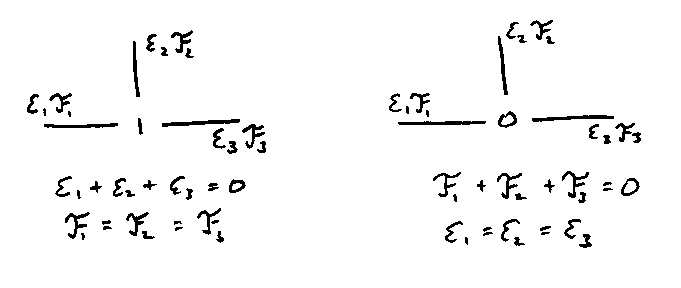
\includegraphics[width=3.5in]{figs14/00309.eps}
\caption{Bond graphs (Figureillustrate ways energy can flow within networks.}\label{BondGraphs}	%<hn>
\end{figure}	%<hn>

 When two ports are connected as in Figure \ref{ConnectedOnePorts}, we can say they are wired in series, but also that they are wired in parallel.  However if three ports are connected together, we need to consider how they are connected.  Series connection means that all the ports have the same flow value and parallel means they share the same effort but have different flows.  Bond Graphs are an abstraction of networks into energy bonds between lumped parameter elements. A ``bond" is a general way of connecting multiple ports together.     Elements are connected at bonds which correspond to Kirchoffs/Newtons laws.	%<hn>

	%<*>
``1 Junction" a bond in which $\sum\limits_i \ef_i = 0$ and $\fl_i = \fl_j$.  For example an electrical series loop or a mass.

``0 Junction" a bond in which $\sum\limits_i \fl_i = 0$ and $\ef_i = \ef_j$.  For example an electrical node (parallel connection) or   mechanical elements which share the same force (Figure \ref{BondGraphs}).

%\end{slide}
%\begin{slide}


An example of an electrical network and its associated Bond Graph is given in Figure \ref{CircuitToBond}.	%<hn>

%
%%%%** Figure 13
\begin{figure}[h]	%<hn>
\centering 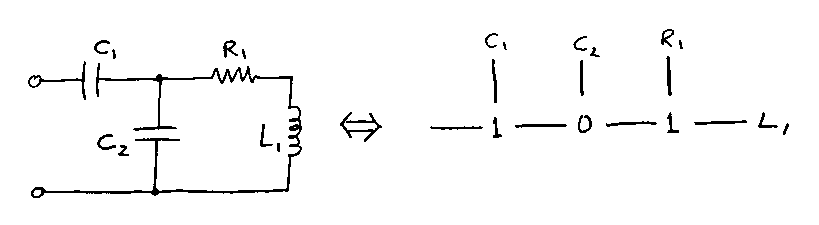
\includegraphics[width=3.5in]{figs14/00314.eps}
\caption{Example of an electrical 1-port and its equivalent bond graph.}\label{CircuitToBond}	%<hn>
\end{figure}	%<hn>


	%<*hn>
%%%%** Section 6.2.2
\subsubsection{Port Hamiltonian Systems (Stramigioli, 2000's)}

Same idea as bond graphs.

	%<*>






%\end{slide}
%\begin{slide}

%%%%%%%%%%%%%%%%%%%%%%%%%%%%%%%%%%%%%%%%%%%%%%%%%%%%%%%%%%%%%%%%%%%%%%%%%%%%%%%%%%%%%%%%%
%%%%** Section 6.3
\subsection{2-Port Network Models}

First, make a key assumption:  Linearity.   In this case, all two port networks can be modeled by	%<hn>
% Linearity

\bq \label{AB}
A  \left [
   \begin{array}{c} \fl_1 \\ \fl_2  \end{array}
   \right]
+
B  \left [
   \begin{array}{c} \ef_1 \\ \ef_2  \end{array}
   \right]
=
0
\eq
Where $A$ and $B$ are $2\times2$ matrices.


%\end{slide}
%\begin{slide}
There are two more useful forms of this equation however known as ``projections" of eqn (\ref{AB}).	%<hn>

% Projections

\bq\label{ZMatrixDef}
   \left [
   \begin{array}{c} \ef_1 \\ \ef_2  \end{array}
   \right]
=
Z  \left [
   \begin{array}{c} \fl_1 \\ \fl_2  \end{array}
   \right]
\eq
where $Z$ is a $2\times2$ ``Impedance Matrix".

and


%\end{slide}
%\begin{slide}

\bq\label{HMatrixDef}
   \left [
   \begin{array}{c} \ef_1 \\ \fl_2  \end{array}
   \right]
=
H  \left [
   \begin{array}{c} \fl_1 \\ \ef_2  \end{array}
   \right]
\eq

where $H$ is a $2\times2$ ``Hybrid Matrix".


%\end{slide}
%\begin{slide}

%%%%** Section 6.4
\subsection{Finding Elements of Z}

First expand eqn(\ref{ZMatrixDef}) to get
\bq
\begin{array}{ll}
\ef_1 = z_{11}\fl_1   +  z_{12}\fl_2    \\
\ef_2 = z_{21}\fl_1   +  z_{22}\fl_2
\end{array}
\eq

Now set some boundary conditions on the network:  $\fl_1  = 0$ or $\fl_2 = 0$.  This allows us to solve for each element of $Z$:	%<hn>


%\end{slide}
%\begin{slide}
\bq
Z =
\left [
\begin{array}{cc}

z_{11} = \left . \frac{\ef_1}{\fl_1}\right |_{\fl_2=0}     &

z_{12} = \left . \frac{\ef_1}{\fl_2}\right |_{\fl_1=0}     \\

z_{21} = \left . \frac{\ef_2}{\fl_1}\right |_{\fl_2=0}     &

z_{22} = \left . \frac{\ef_2}{\fl_2}\right |_{\fl_1=0}

\end{array}
\right ]
\eq

{\bf Note: } The boundary conditions ( $\fl_1  = 0$ or $\fl_2 = 0$) which allow us to solve for the elements of $Z$ are not only mathematically useful, they define simple physical experiments which can be peformed on the 2-port network:	%<hn>


%\end{slide}
%\begin{slide}
\vspace{0.25in}

\begin{tabular}{|c|c|c|c|}
\hline
             &           &      Mechanical                 &  Electrical           \\
\hline
Flow:        &  $\fl=0$  &      motion blocked             &  open circuit         \\
\hline
Effort:      &  $\ef=0$  &      free motion                &  short circuit         \\
\hline
\end{tabular}

\vspace{0.25in}


%\end{slide}
%\begin{slide}

%%%%** Section 6.5
\subsection{Finding Elements of H}
% \begin{example}

Exercise:   Find the elements of $H$ (eqn(\ref{HMatrixDef})


%\end{slide}
%\begin{slide}

%\vspace{3.25in}

	%<*sn>
First expand eqn(\ref{HMatrixDef}) to get
\bq \label{HExpanded}
\begin{array}{ll}
\ef_1 = h_{11}\fl_1   +  h_{12}\ef_2    \\
\fl_2 = h_{21}\fl_1   +  h_{22}\ef_2
\end{array}
\eq

	%<*n>
Now set some boundary conditions on the network:  $\fl_1  = 0$ or $\ef_2 = 0$.  This allows us to solve for each element of $H$:


\bq
H =
\left [
\begin{array}{cc}

h_{11} = \left . \frac{\ef_1}{\fl_1}\right |_{\ef_2=0}     &

h_{12} = \left . \frac{\ef_1}{\ef_2}\right |_{\fl_1=0}     \\

h_{21} = \left . \frac{\fl_2}{\fl_1}\right |_{\ef_2=0}     &

h_{22} = \left . \frac{\fl_2}{\ef_2}\right |_{\fl_1=0}

\end{array}
\right ]
\eq
% \end{example}
	%<*>

%\end{slide}
%\begin{slide}

So far we have treated the $Z$ and $H$ matrix elements $h_{ij}$ and $z_{ij}$ as scalar real numbers.  If we are able to model the system with differential equations however, we can use LaPlace transforms and the matrix elements become functions of complex frequency, $s$.   However for simplicity we will usually omit the $(s)$.	%<hn>










%\end{slide}
%\begin{slide}
%%%%%%%%%%%%%%%%%%%%%%%%%%%%%%%%%%%%%%%%%%%%%%%%%%%%%%%%%%%%%%%%%%%%%%%%%%%%%%%%%%%%%%%%%
%%%%** Section 7
\section{Models of Teleoperation}

%%%%** Section 7.1
\subsection{Interpretation of the H Parameters}

Recall that we have the analogies:

\begin{centering}
Velocity $\leftrightarrow$ Current \\
Force    $\leftrightarrow$ Voltage\\
\end{centering}

With Impedance Control from robotic manipulation, we study the control of mechanical impedance at the contact point between robot and environment: a port.  Both the robot and the environment are one-ports which are conected.	%<hn>


%%%%** Figure 14
\begin{figure}[h]	%<hn>
\centering 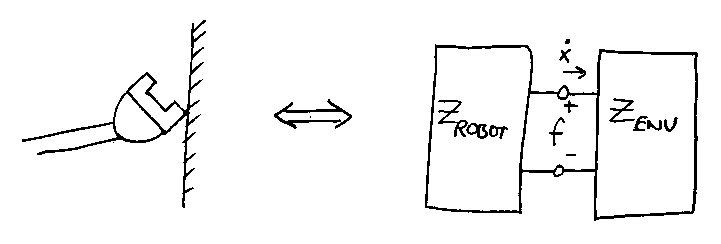
\includegraphics[width=3.5in]{figs14/00319.eps}
\caption{Contact between a robot manipulator and environment (Left) is a port at which mechanical energy can flow back and forth between the robot and environment. It is represented as two one-ports connected together (Right).}\label{RobotEnvContact}	%<hn>
\end{figure}	%<hn>


For a bilateral teleoperation system  (Figure \ref{BasicBilateralTeleop}) we have two contact points and therefore use a two-port model.	%<hn>


%%%%** Figure 15
\begin{figure}[h]	%<hn>
\centering 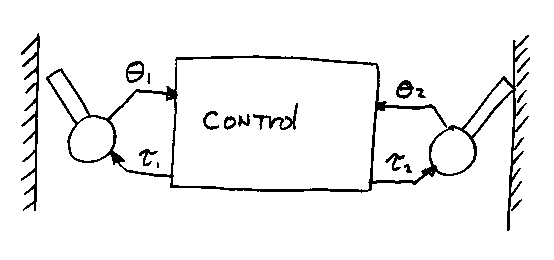
\includegraphics[width=3.5in]{figs14/00320.eps}
\caption{Simple bi-lateral teleoperation system has two ports: the leader and follower robots (here shown as a completely symmetrical system) contact two separate environments. The human operator is usually shown in place of the left side environment.}\label{BasicBilateralTeleop}	%<hn>
\end{figure}	%<hn>



%\end{slide}
%\begin{slide}

We then use the $H$ parameters (i.e. the elements of $H$) to study the system.   Let's express the definition of the $h_{ij}$ elements in terms of the mechanical effort and flow variables:

\bq\label{h11}
h_{11} = \left . \frac{f_1}{\dot{x}_1}\right |_{f_2=0}
\eq
\bq\label{h12}
h_{12} = \left . \frac{f_1}{f_2}\right |_{\dot{x}_1=0}
\eq
\bq\label{h21}
h_{21} = \left . \frac{\dot{x}_2}{\dot{x}_1}\right |_{f_2=0}
\eq
\bq\label{h22}
h_{22} = \left . \frac{\dot{x}_2}{f_2}\right |_{\dot{x}_1=0}
\eq


%\end{slide}
%\begin{slide}

Note that $h_{11}$ (eqn (\ref{h11})) is an effort over a flow and thus it is an impedance.    Furthermore, we observe:	%<hn>
\begin{itemize}
  \item $h_{11}$ involves only variables at the input port.
  \item Because of the applicable boundary condition, $f_2=0$, $h_{11}$ can only be measured or computed when the output port is in free motion (e.g. not in contact fro which $f_2=0$).
  \item $h_{11} = z_{11}$
\end{itemize}
With these considerations, $h_{11}$ represents the input impedance (i.e. resistance felt by the human operator) when the follower is not touching anything.

Similarly, $h_{12}$ is a ratio of the two forces at the ports.   We observe:

\begin{itemize}
  \item $h_{12}$ is dimensionless.
  \item $h_{12}$ represents a gain or transfer function from follower force to leader force.
  \item $h_{12}$ characterizes the nature of force feedback to the operator.
  \item The boundary condition for $h_{12}$ requires that it be measured or computed with the leader device locked so that it cannot move.
\end{itemize}

Extending this reasoning to the other $H$ parameters, we have

\vspace{0.25in}
\begin{tabular}{ll}
\hline
$h_{11}$        &    Input Impedance with Free Follower Motion.   \\
$h_{12}$        &    Force Feedback Gain with Locked Leader, $\lambda_f$. \\
$h_{21}$        &    Forward Velocity Gain with Free Follower Motion,  $\lambda_p$.   \\
$h_{11}$        &    Input impedance with Free Follower Motion.   \\
\hline
\end{tabular}


%\end{slide}
%\begin{slide}

\vspace{0.25in}
Where we have also defined $\lambda_p$ and $\lambda_f$ to conveniently denote the position/velocity and force scales respectively.	%<hn>

%\end{slide}
%\begin{slide}

%%%%** Section 7.2
\subsection{Equivalent Circuits}

The mathematical form of the $H$ and $Z$ matrices suggest that there is an equivalent circuit model which can represent any two port network.   This is analogous to Thevenin and Norton forms of the one-port network.	%<hn>

%
%%%%** Figure 16
\begin{figure}[h]	%<hn>
\centering 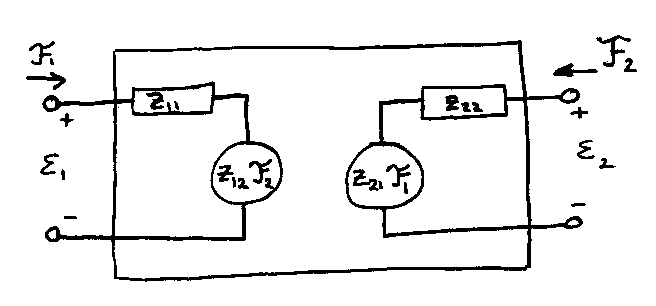
\includegraphics[width=3.5in]{figs14/00310.eps}
\caption{Equivalent circuit two-port based on the impedance matrix, $Z$.}\label{ZEquivTwoPort}	%<hn>
\end{figure}	%<hn>


The impedance matrix creates an equivalent circuit with a Thevenin style network at each port (Figure \ref{ZEquivTwoPort}).  The effort souces are controlled based on the flow variable in the other port.	%<hn>

%
%%%%** Figure 17
\begin{figure}[h]	%<hn>
\centering 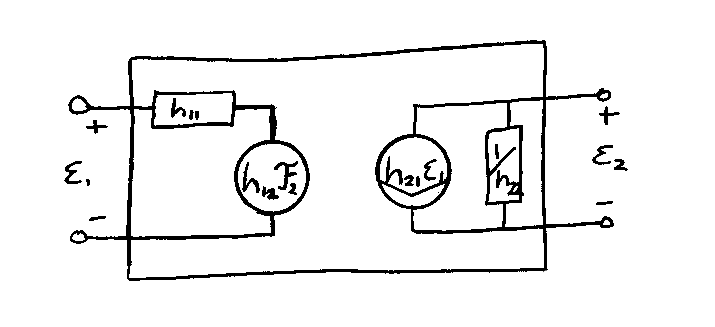
\includegraphics[width=3.5in]{figs14/00311.eps}
\caption{Equivalent circuit two-port based on the hybrid parameters.}\label{HEquivTwoPort}	%<hn>
\end{figure}	%<hn>


The hybrid matrix representation lends itself more naturally to a different equivalent circuit with the same circuitry on port 1, but a Norton form on port 2 (Figure \ref{HEquivTwoPort}).	%<hn>

Remember that both $H$ and $Z$ forms can represent any network, and transformations exist which can translate between the forms (see a book on network theory).




%%%%%%%%%%%%%%%%%%%%%%%%%%%%%%%%%%%%%%%%%%%%%%%%%%%%%%%%%%%%%%%%%%%%%%%%%%%%%%%%%%%%%%%%%
%%%%** Section 8
\section{Kinesthesia}
\begin{quotation}
\noindent
``The sensation of {\bf movement} or {\bf stress} in muscles, tendons, and joints."\\
Random House Dictionary.
\end{quotation}


Two components:  ``Movement" and ``Stress".

Clearly this channel is used in natural manipulation.    How can kinesthesia be supported in telemanipulation?


%\end{slide}
%\begin{slide}

Approaches:
\begin{itemize}

\item Send force from leader to follower and force from follower to leader.
\item Send position from leader to follower, force from follower to leader (``force feedback").
\item Send position in both directions.

\end{itemize}

Which is best?   What is our analytical approach?

How do we analyze a control system where each end is both an input and output?





%\end{slide}
%\begin{slide}
%%%%%%%%%%%%%%%%%%%%%%%%%%%%%%%%%%%%%%%%%%%%%%%%%%%%%%%%%%%%%%%%%%%%%%%%%%%%%%%%%%%%%%%%%%%%
%%%%** Section 9
\section{Ideal Bilateral teleoperator: Massless Stick}

First let's put these ideas to work on bilateral kinesthetic systems.    First consider a rigid massless stick with which a human is pushing on the environment  in the axial direction (Figure \ref{MasslessStick}).


%%%%** Figure 18
\begin{figure}[h]	%<hn>
 \centering 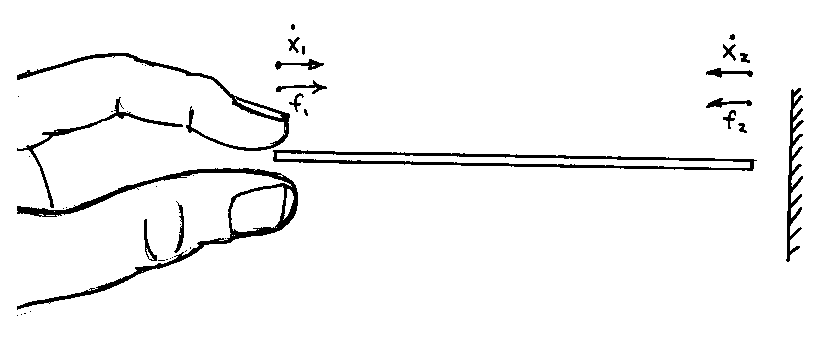
\includegraphics[width=3.5in]{figs14/00312.eps}
\caption{Rigid and massless stick held by operator at one end and touching an environment at the other can be analyzed as a two port system.}\label{MasslessStick}	%<hn>
\end{figure}	%<hn>


Clearly the ports are the two ends of the stick.   Following Section \ref{Signs}, we assign signs to the effort and flow variables as follows:
\begin{enumerate}
\item Positive direction for velocity is into the ends of the stick, i.e. to the right on the left end and to the left on the right end.
\item When power flows into the stick, force must be in the same direction as the velocity, so force has the same sign.
\end{enumerate}

{\bf Note:}

Designation of ``Leader" and ``Follower" ends is completely arbitrary.

With a massless stick, we have a direct kinesthetic correspondance between hand force/velocity and environment force/velocity.


%\end{slide}
%\begin{slide}

%%%%** Section 9.1
\subsection{Hybrid Matrix of Massless Stick}

With the correct sign conventions, and 
using intuition extrapolated from real-world experiences using low-mass sticks, 
we write
\bq
\dot{x_1} = -\dot{x_2} \qquad \mathrm{and} \qquad f_1 = f_2
\eq

({\bf Note:} $f_1$ and $f_2$ must represent forces exerted on the stick.  In a single global coordinate system they would be normally in opposite directions. However with the two coordinate systems we have chosen for the two ends of the stick, compressive forces on the stick would have the same sign.)

Now let's derive the $H$ parameters using equations (\ref{h11} --- \ref{h22}):


\bq
h_{11} = \left . \frac{f_1}{\dot{x}_1}\right |_{f_2=0}  =  0
\eq
\bq
h_{12} = \left . \frac{f_1}{f_2}\right |_{\dot{x}_1=0}   = 1
\eq
\bq
h_{21} = \left . \frac{\dot{x}_2}{\dot{x}_1}\right |_{f_2=0}  = -1
\eq
\bq
h_{22} = \left . \frac{\dot{x}_2}{f_2}\right |_{\dot{x}_1=0}     0
\eq

or

\bq\label{HIdeal}
% H_{ideal}  = \left [
% \begin{array}{cc}
% 0 & 1 \\ -1 & 0
% \end{array}
% \right]
H_{ideal}  = \begin{bmatrix}
0 & 1 \\ -1 & 0
\end{bmatrix}
\eq

Note that applying similar analysis to the $Z$ matrix give us

\bq
Z_{ideal} = \left [
\begin{array}{cc}
\infty & \infty \\ \infty & \infty
\end{array}
\right] 
\eq

The different two port models do not always exist.

%%%%%%%%%%%%%%%%%%%%%%%%%%%%%%%%%%%%%%%%%%%%%%%%%%%%%%%%%%%%%%%%%%%%%%%%%%%%%%%%%%%%%%%%%%%%%%%%%%%%%%%%%%
%%%%** Section 10
\section{Position error-based Leader-Follower Teleoperation}

%
%%%%** Figure 19
\begin{figure}[h]	%<hn>
\centering \includegraphics[width=3.5in]{figs14/00313.eps}
\caption{Classical leader-follower bi-lateral teleoperation control system.  Leader and follower devices are represented as Thevenin equivalent circuits.  Mechanical impedances represent viscous and inertial properties of the devices such as motor inertia. $f_i$: forces (efforts), $\dot{x}_i$: velocities (flows)}\label{ClassicalLeaderFollower}	%<hn>
\end{figure}	%<hn>

We now consider the original bilateral control method (going back to Ray Goertz) in which position error between leader and follower is used to generate a force feedback signal (Figure \ref{ClassicalLeaderFollower}).  Here we have a diagram showing the leader and follower units as Thevenin equivalent one-ports.  These are reasonable models of electric motor driven motion axes.  The source in each one-port is a dependent effort source such that
\bq
f_2 = f_3 = (\dot{x}_1 + \dot{x}_2)G
\eq

%\end{slide}
%\begin{slide}

\bq\label{HMatrixDef2}
   \left [
   \begin{array}{c} f_1 \\ \dot{x}_4  \end{array}
   \right]
=
H_{LF}  \left [
   \begin{array}{c} \dot{x}_1 \\ f_4  \end{array}
   \right]
\eq

You can show:


\bq\label{HClassical}
H_{LF}  = \left [
\begin{array}{cc}
Z_3 + G\left[ 1- \frac{G}{Z_3+G} \right ]
&
\frac{G}{Z_3+G}
\\
\frac{-G}{Z_3+G}
&
\frac{1}{Z_3+G}
\end{array}
\right]
\eq


%\end{slide}
%\begin{slide}

Example solution:

\bq
h_{12} = \left . \frac{f_1}{f_4}\right|_{\dot{x}_1=0}
\eq
when $\dot{x}_1 = 0$, $f_1 = f_2 = \dot{x}_4G$.
then we have
\bq
\dot{x}_2 = \frac{f_4-f_3}{Z_3} =
\frac{1}{Z_3}f_4 - \dot{x}_2\frac{G}{Z_3}
\eq




%\end{slide}
%\begin{slide}

Now, if we are given the task to design $G$ in order to achieve ideal behavior (equation \ref{HIdeal}) we can try to make $|G|$ as large as possible over some frequency range, but ideal teleoperation will never be achieved because
\bq
h_{11} \rightarrow Z_3 \qquad \mathrm{as} \quad |G| \rightarrow \infty
\eq


%%%%** Section 11
\section{Forward Flow Leader Follower Teleoperation}

(future material)








%\end{slide}
%\begin{slide}
%%%%%%%%%%%%%%%%%%%%%%%%%%%%%%%%%%%%%%%%%%%%%%%%%%%%%%%%%%%%%%%%%%%%%%%%%%%%%%%%%%%%%%%%%%%%
%%%%** Section 12
\section{Lever Bilateral teleoperator: Artist's Paintbrush}


%%%%** Figure 20
\begin{figure}[h]	%<hn>
\centering 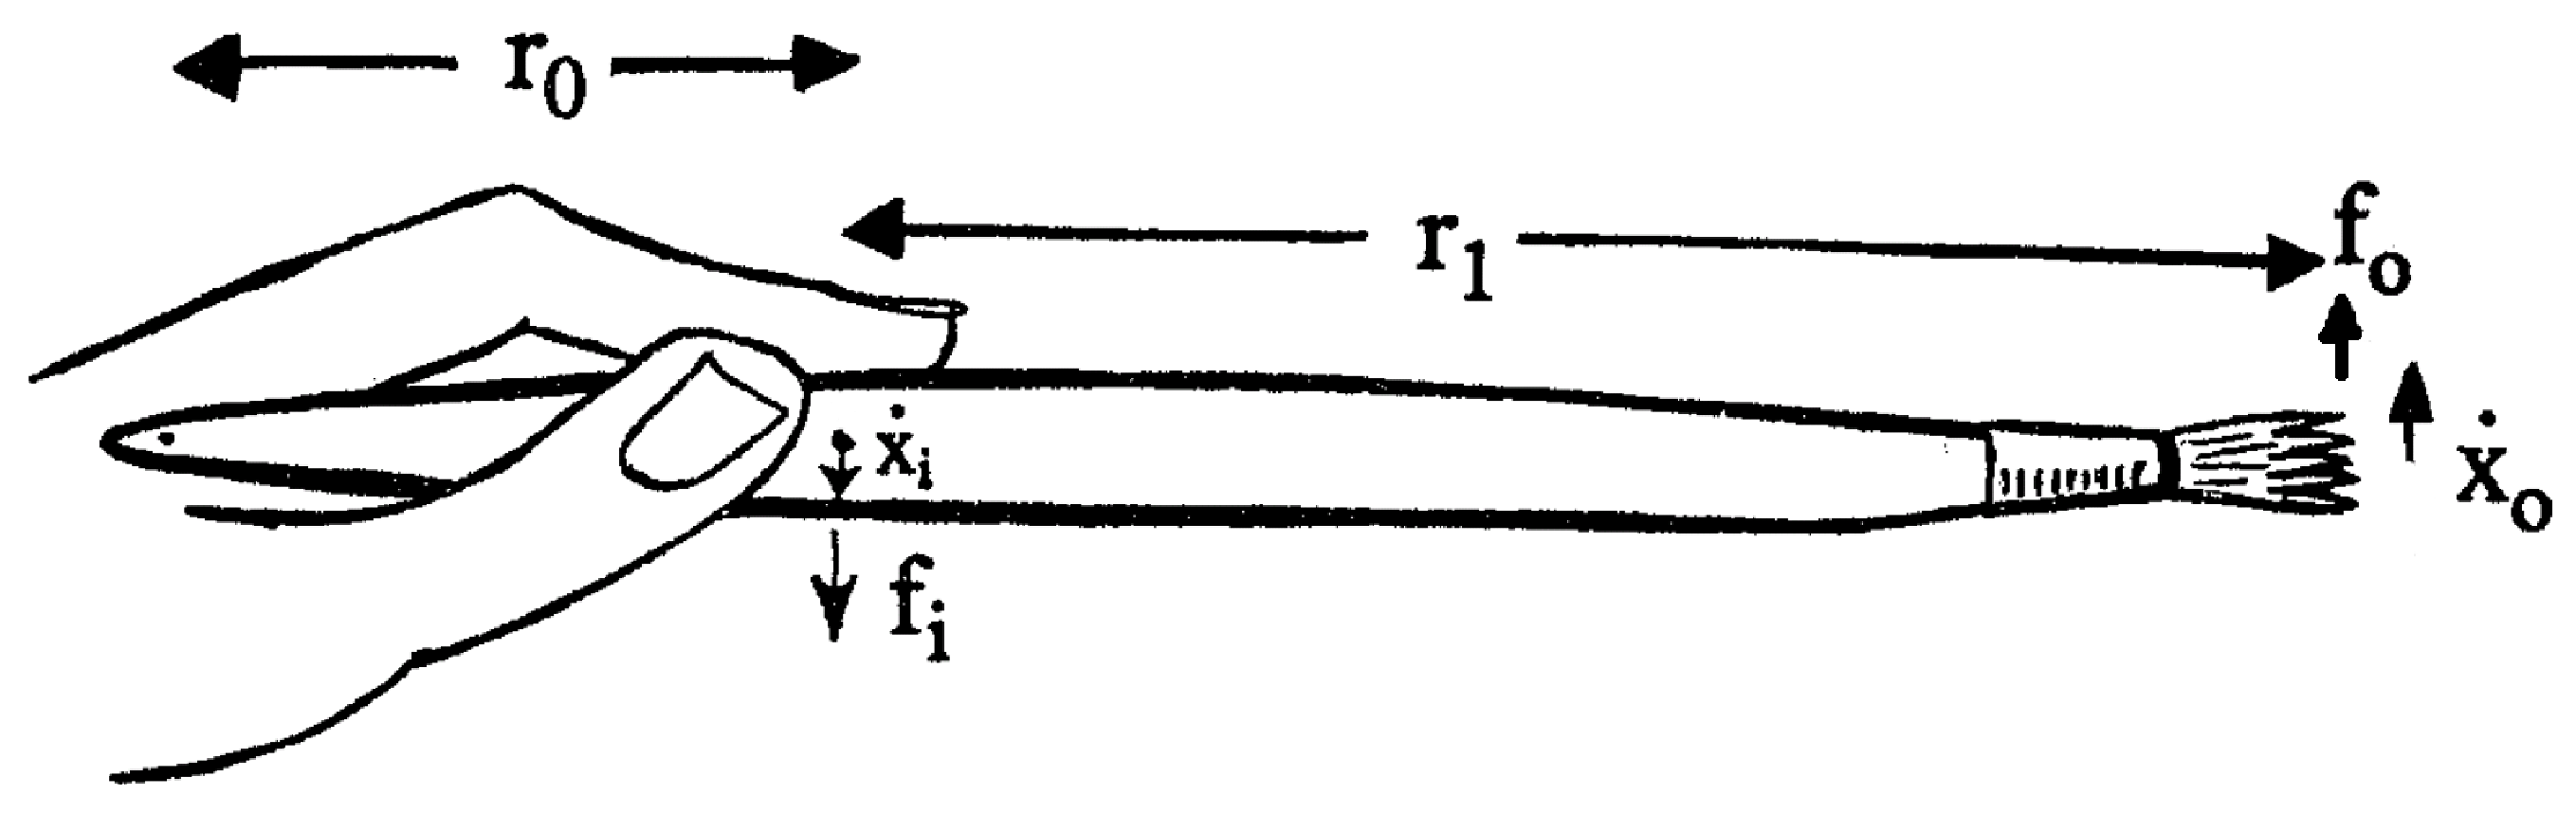
\includegraphics[width=5.5in]{figs14/paintbrush.eps}	%<hn>
% \centering 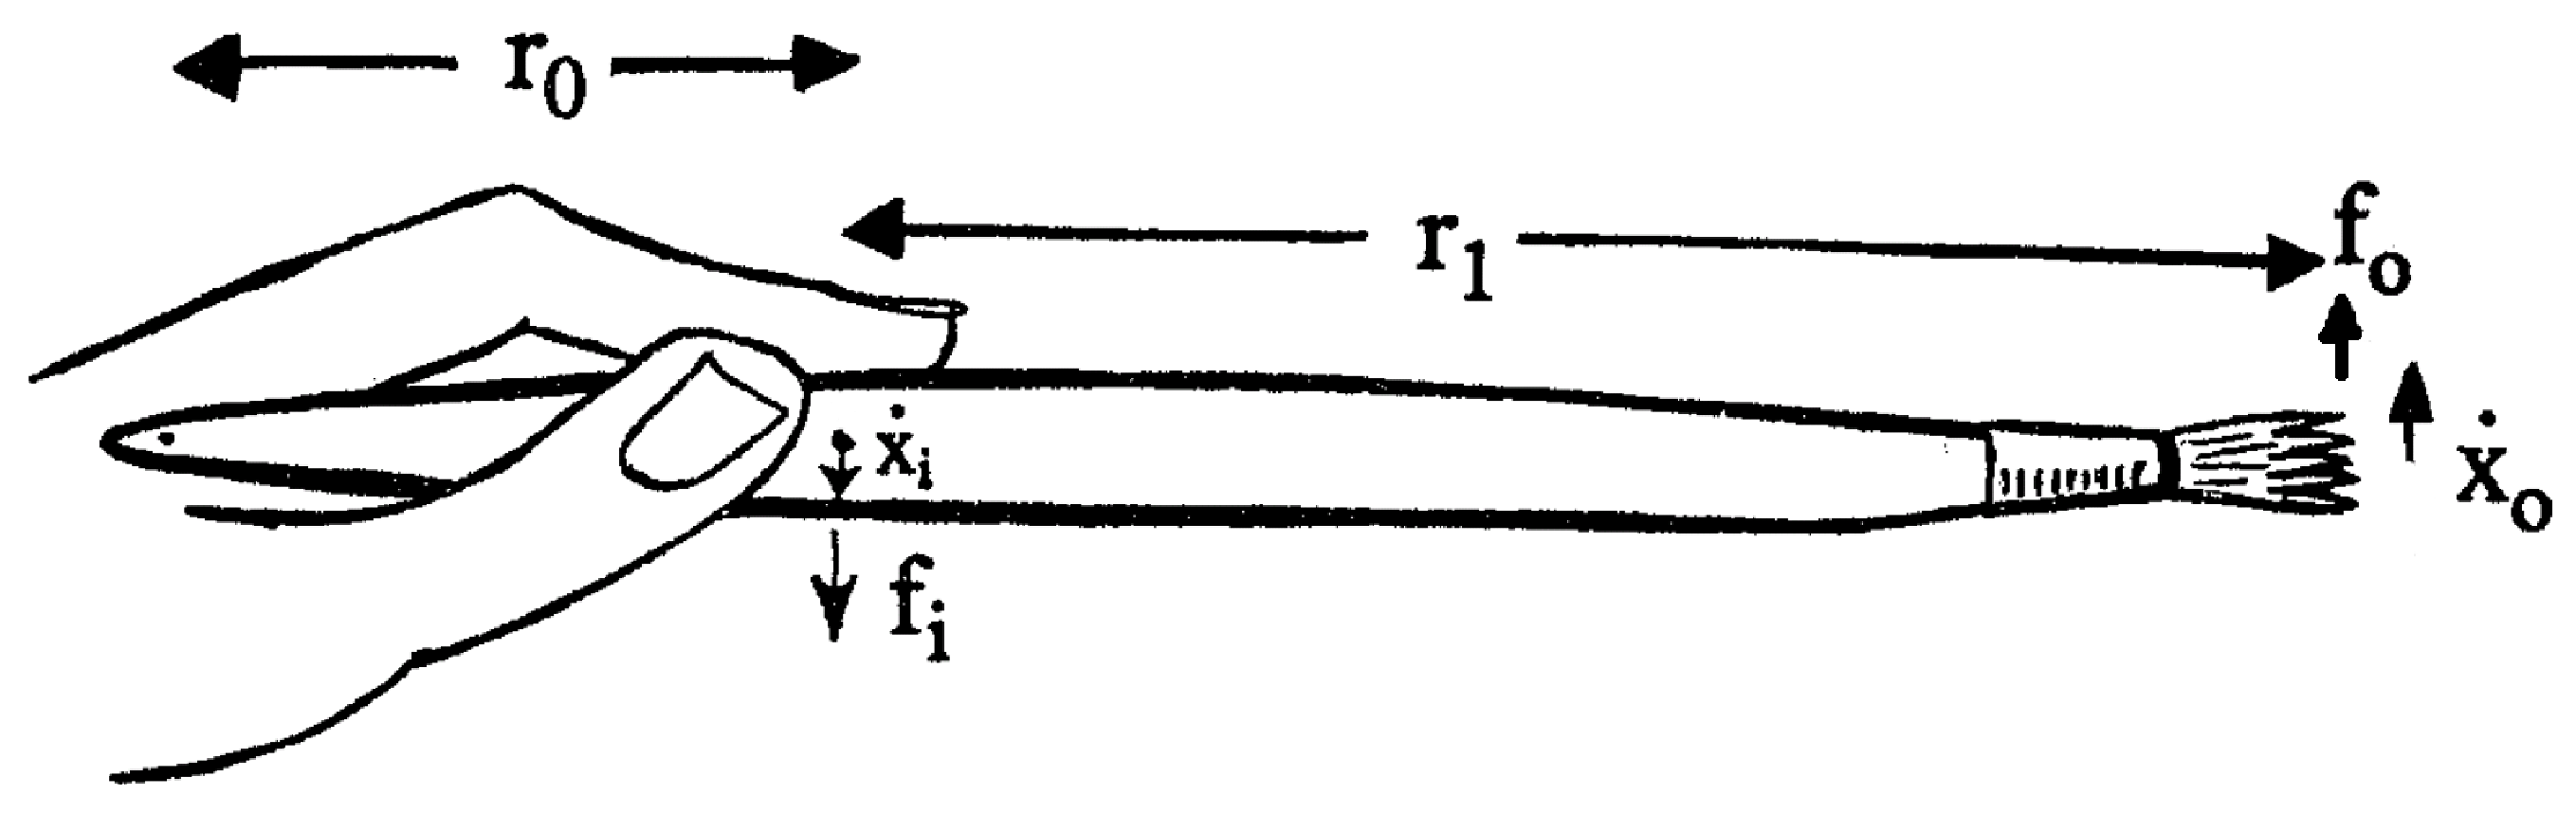
\includegraphics[width=3.5in]{figs14/paintbrush.eps}
\caption{An artist's paintbrush will serve as an example of how two-port modeling can be used to study tool use.)}\label{PaintBrush}	%<hn>
\end{figure}	%<hn>


Consider a long artist's paint brush (Figure \ref{PaintBrush}).  The following section will analyze such a tool with two-port network theory to gain some informal insight into how a brush might be used by the painter for different effects. This time we assume the stick has some mass, expressed in terms of a linear density, $\rho$ which describes the mass per unit of length.


%\end{slide}
%\begin{slide}

%%%%** Section 12.1
\subsection{H Matrix of Paintbrush}

We leave it as an exercise to the reader to derive the following hybrid matrix for the brush.

\bq\label{HBrush}
H_{ideal}  = \left [
\begin{array}{cc}
\frac{\rho(r_0+r_1)^2s}{2}
&
\frac{r_0+r_1}{r_0}
\\
-(\frac{r_0+r_1}{r_0})
&
\frac{r_1s}{k}
\end{array}
\right]
\eq

Where $\rho$  is the linear density of the brush ($\frac{\partial m}{\partial x}$),
$k$ is the spring constant for bending the brush, and $s$ is the LaPlace transform variable.

%\end{slide}
%\begin{slide}

Here's how the $h$ parameters describe physical phenomena in the brush.

\bq\label{HBrush2}
H_{ideal}  = \left [
\begin{array}{cc}
\mathrm{Brush \quad inertial \quad behavior}
&
\mathrm{Mechanical \quad Advantage}
\\
\mathrm{Mechanical \quad Advantage}
&
\mathrm{Spring-like \quad Bending}
\end{array}
\right]
\eq

As for any system based on a lever/fulcrum,
\bq
\lambda_f =  h_{12} = \frac{r_0+r_1}{r_0} \qquad
\lambda_p = -h_{21} = -\frac{r_0+r_1}{r_0}
\eq
%\end{slide}
%\begin{slide}

We can also show that when using the paintbrush, the impedance ``seen" by the paint, in other words the combined effects of the artist impedance and brush impedance, $Z_{AB}$, is

\bq
Z_{AB} = Z_A \left( \frac{r_0}{r_0+r_1} \right)^2
\eq

By varying his/her grip on the brush, the artist changes $r_0$ and $r_1$, keeping their total constant.

Let's consider extreme cases,

1)  $r_0 \rightarrow 0$

In this case $Z_{AB} \rightarrow 0$.    Recall that when impedance is 0, we have an ideal force (effort) source.


2)  $r_1 \rightarrow 0$

In this case $Z_{AB} \rightarrow Z_A$.     Recall that when impedance is $\infty$, we have an ideal velocity/position (flow) source.  Although the artist cannot achieve infinite impedance, $Z_A$ may be the highest impedance that the artist can achieve.

%\end{slide}
%\begin{slide}


%\end{slide}
%\begin{slide}
%%%%%%%%%%%%%%%%%%%%%%%%%%%%%%%%%%%%%%%%%%%%%%%%%%%%%%%%%%%%%%%%%%%%%%%%%%%%%%%%%%%%%%%%%%%%%%
%%%%** Section 13
\section{Scaled Bi-Lateral Teleoperation}

For many applications, we might want to scale force and position up or down from a comfortable range for the human operator to some other domain ideal for a task.  For example in a micro surgery system we might want to scale down the operator's motion and scale up force feedback to the operator so that tiny delicate tissues are easier to feel.	%<hn>

Already a huge range of scale factors ($10^{10}$) have been implemented in teleoperation (Figure \ref{ScaleRange})

%%%%** Figure 21
\begin{figure}[h]	%<hn>
\centering 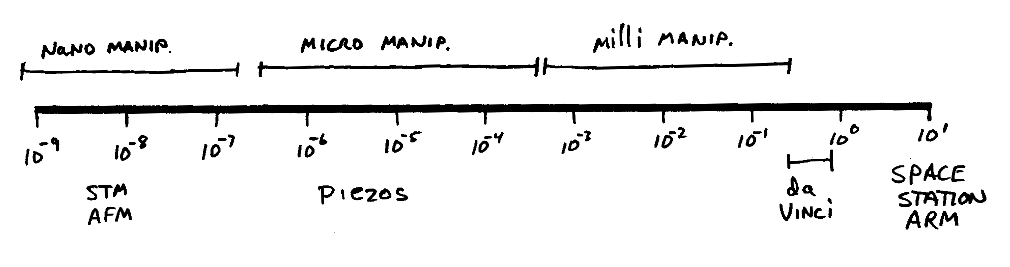
\includegraphics[width=4.5in]{figs14/00317.eps}
\caption{A huge range of scale factors has been used in teleoperation systems that have been developed.}\label{ScaleRange}	%<hn>
\end{figure}	%<hn>

%%%%** Section 13.1
\subsection{Scaled Mechanical Impedance}

Consider $\lambda_p \neq 1$ and $\lambda_f \neq 1$.  If the follower robot is in contact with a mechanical impedance $Z_E$, what is the impedance experienced or felt by the human operator?  We denote this impedance $Z_{felt}$ and illustrate where it is measured and defined in Figure \ref{Zfelt}.
%                      (19)
%%%%** Figure 22
\begin{figure}[h]	%<hn>
\centering 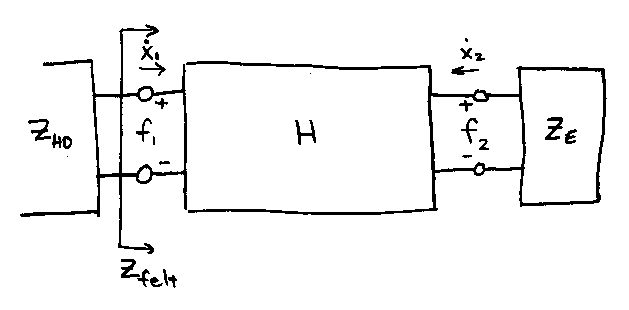
\includegraphics{figs14/00318.eps}
\caption{Two-port model of scaled teleoperation illustrating the impedance, $Z_{felt}$, experienced by the operator when contact with an environment is mediated by a scaled teleoperator.}\label{ScaledTwoPort}\label{Zfelt}	%<hn>
\end{figure}	%<hn>


\bq
Z_{felt} = \frac{f_1}{\dot{x}_1}
\eq
Expanding equation (\ref{HMatrixDef2}), and solving for $f_2$, we have
\bq
f_1 = h_{11}\dot{x}_1 + h_{12}(-\dot{x}_2 Z_E)
\eq
and
\bq
\dot{x_2} = h_{21}\dot{x}_1 + h_{22}(-\dot{x}_2Z_E)
\eq
Solving for $\dot{x}_1$,
\bq
\dot{x}_1 = h_{21}\frac{\dot{x}_1}{1+Z_Eh_{22}}
\eq
and
\bq
f_1       = h_{11}\dot{x}_1 - \frac{h_{12}h_{21}}{1+Z_Eh_{22}} Z_E\dot{x}_1
\eq
With these two components, we get:
\bq
Z_{felt} =  h_{11} -  \left [ \frac{h_{12}h_{21}}{1+Z_Eh_{22}} \right ] Z_E
\eq
or equivalently
\bq
Z_{felt} =  h_{11} + \left [ \frac{\lambda_p\lambda_f}{1+Z_Eh_{22}} \right ] Z_E
\eq

% {\bf Reality Check: } verify that the term
%\[
%\left [ \frac{\lambda_p\lambda_f}{1+Z_Eh_{22}} \right ]
%\]
%is dimensionless.
	%<*>

If the leader and follower mechanisms are perfect or idealized (that is they have no losses due to friction or compliance), then	%<hn>
ideally $h_{11} = 0$ and $Z_E h_{22} = 0$.  Giving
\bq
\boxed{   Z_{felt} = \lambda_p\lambda_f Z_E     }
\eq

%\end{slide}
%\begin{slide}

%%%%** Section 13.2
\subsection{Power Gain from Leader to Follower}

It can be shown\footnote{ B. Hannaford,  'Kinesthetic Feedback Techniques in Teleoperated Systems,'  In ``Advances in Control and Dynamic Systems", pp. 1-32, C. Leondes, Ed., Academic Press, San Diego, 1991.} that for the system of Figure \ref{ScaledTwoPort},

\bq
P_1 = -P_4\left(-\frac{h_{21}}{h_{12}}+\frac{2h_{11}h_{22}}{h_{21}^2}\right)
     + f_2^2h_{22}\left(\frac{h_{21}}{h_{12}}+\frac{h_{11}h_{22}}{h_{21}^2}\right)
     + \dot{x}_2^2\frac{h_{11}}{h_{21}^2}
\eq
where $P_1$ is the power going into port 1 and $P_4$ is the power going into port 2.
Let us assume an ideal scaled teleoperator having hybrid matrix
\bq
H = \left [
\begin{array}{cc}
0   & \lambda_f \\ -\lambda_p & 0
\end{array}
\right]
\eq
Then we have
\bq
P_1 = -P_4\frac{\lambda_p}{\lambda_f}
\eq
Thus, power at the human operator side is scaled relative to the environment side by $\frac{\lambda_p}{\lambda_f}$.

%\end{slide}
%\begin{slide}



\section{Stability}
\subsection{Basic Linear Control Theory}
\subsection{Passivity}
\subsection{Time Delay}


\section{Lawrence Four-Channel Architecture}


%%%%** Section 13.3
\subsection{Scaled Teleoperation Conclusions}	%<hn>


%%%%** Figure 23
\begin{figure}[h]	%<hn>
\centering 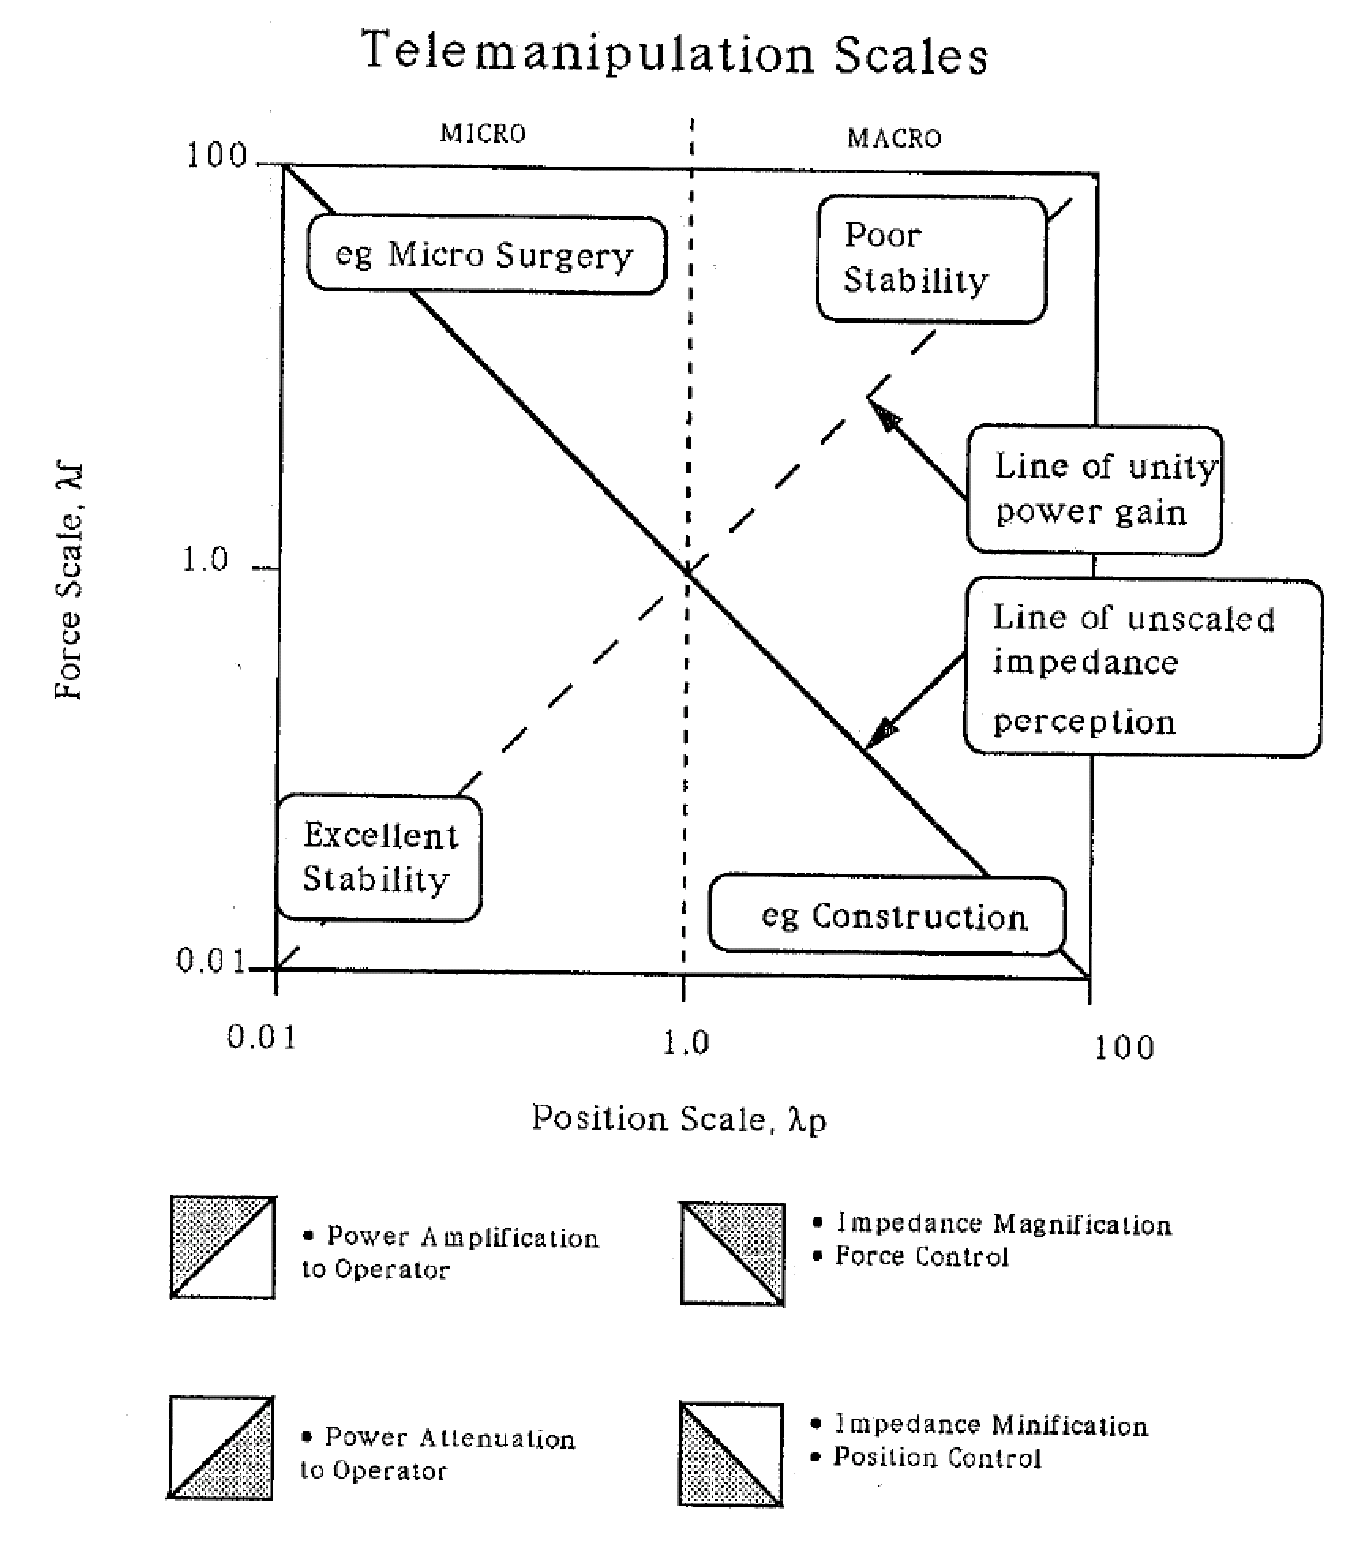
\includegraphics[width=5in]{figs14/lambdachart.eps}
\caption{Properties of bi-lateral teleoperators depending on position and forces scales: $\lambda_p$ and $\lambda_f$.}\label{LambdaChart}	%<hn>
\end{figure}	%<hn>


We have the following observations
sumarized in Figure \ref{LambdaChart}.	%<hn>
\begin{itemize}
  \item For all levers, $\lambda_p = \lambda_f$.

   \item If $\lambda_p\lambda_f > 1$, environment impedance is magnified to the operator.

   \item If $\lambda_p\lambda_f < 1$, environment impedance is reduced   to the operator.

   \item If $\frac{\lambda_p}{\lambda_f} > 1$ power is amplified from the environment to operator  and attenuated from operator to environment.

   \item If $\frac{\lambda_p}{\lambda_f} < 1$ power is attenuated from the environment to operator  and amplified from operator to environment.
\end{itemize}

%\end{slide}
	%<*>

